
\chap{Rahasia Arwah-arwah di Api Penyucian}
\begin{center}\large
Wawancara dengan Maria Simma dari Austria
\normalsize
\end{center}
\setlength{\parindent}{0cm}
\renewcommand{\figurename}{~}

\begin{wrapfigure}{l}{3cm}
\centering
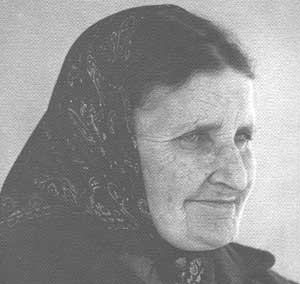
\includegraphics[scale=0.25]{gambar/simma.jpg}
\caption{\scriptsize\mbox{Maria Simma (1915-2004)}\normalsize}
\end{wrapfigure}

Saat ini, sangat sedikit yang diajarkan di kelas katekismus reguler tentang Api Penyucian, tentang penderitaan arwah-arwah agar benar-benar murni untuk dapat masuk ke dalam Kerajaan Surga. Namun Api Penyucian dan penderitaan arwah-arwah  adalah sangat nyata.

Sejak 1940 (ia saat itu berusia 25), seseorang yang istimewa, bernama Maria Simma, telah memiliki kunjungan rutin dari jiwa-jiwa di Api Penyucian untuk menjelaskan penderitaan mereka dan untuk meminta doa dan Misa agar dibebaskan dari Api Penyucian. Uskup setempat dan pastor paroki mengatakan bahwa ia boleh membuat kunjungan ini dikenal selama tidak ada kesalahan teologis.

Suatu hari, Suster Emmanuel Maillard, seorang biarawati Perancis yang menjalankan tugas kerasulan dan mendukung Penampakan Bunda Maria di Medjugorje, menemukan buku Maria Simma, yang berjudul \textit{The Souls in Purgatory told Me...} yang berupa mengenai arwah-arwah di Api Penyucian dan membacanya dengan penuh minat: ``Saya sungguh terpesona karena isinya menyangkut kesaksian-kesaksian baru-baru ini dan juga menjelaskan dengan baik tentang doktrin-doktrin Gereja Katolik tentang topik tersebut. Langsung, saya menulis kepada editor yang mengatakan kepada saya bahwa Maria Simma masih hidup. Dengan cepat, saya menghubungi dia, dan dia setuju untuk bertemu saya untuk menjawab pertanyaan saya, yang banyak!''

Wawancara ini berlangsung tahun 1997 di rumah Maria di Sonntag, sebuah desa yang sangat indah di Pegunungan Vorarlberg di Austria. Berikut ini adalah kutipan dari wawancara Suster Emmanuel (SE) dari Medjugorje dengan Maria Simma (MS), diambil dari sebuah buku kecil berjudul: \textit{The Amazing Secret of the Souls in Purgatory}, yang diterbitkan oleh Queenship Publishing Co, PO Box 220, Goleta, CA 93116, USA 

\noindent{\textit{(Catatan: Maria Simma meninggal pada 16 Maret 2004, di Sonntag, pada usia 89.)}}


\subsection*{PERTAMA KALINYA}
\newcommand{\BSE}[1]{\begin{itemize} \item[SE:] \textbf{#1} \end{itemize}}
\newcommand{\BMS}[1]{\begin{itemize} \item[MS:] \textit{#1} \end{itemize}}

\BSE{Maria, bisakah Anda menceritakan kepada kami bagaimana Anda pertama kali dikunjungi oleh arwah dari Api Penyucian?} 
\BMS{Ya, waktu itu tahun 1940. Suatu malam, sekitar jam 3 atau 4 pagi, saya mendengar seseorang masuk ke dalam kamar tidur saya. Hal itu membuat saya terbangun. Saya mencari-cari siapa gerangan yang dapat masuk ke dalam kamar tidur saya.}

\BSE{Apakah Anda ketakutan?}
\BMS{Tidak, saya tidak takut sama sekali. Bahkan sewaktu saya masih kecil, ibu saya mengatakan bahwa saya anak yang spesial karena saya tidak pernah merasa takut.}

\BSE{Jadi, malam itu... ceritakanlah kepada kami!}
\BMS{Saya melihat seorang yang sama sekali tidak saya kenal. Dia berjalan bolak-balik secara perlahan. Saya berseru keras kepadanya: "Bagaimana Anda dapat masuk kesini? Pergilah!" Tetapi dia terus berjalan dengan tidak sabar disekeliling kamar tidur, seolah-olah dia tidak mendengar perkataan saya. Jadi saya kembali bertanya: "Apa yang sedang Anda lakukan?" Tetapi karena dia tetap tidak memberi jawaban, saya turun dari ranjang dan mencoba menjamahnya, tetapi saya hanya menjamah udara kosong. Tidak ada apa-apa disana. Jadi saya kembali ke ranjang, tetapi kembali saya mendengarnya berjalan bolak-balik.
\\
Saya membayangkan bagaimana saya bisa melihat lelaki ini tetapi saya tidak dapat menjamahnya. Saya bangkit kembali untuk mencoba memegang orang itu dan menghentikan dia; kembali saya hanya merasakan kekosongan belaka.
\\
Bingung, saya lantas kembali ke ranjang. Dia tidak muncul kembali, tetapi saya tidak dapat kembali tidur. Hari berikutnya setelah Misa, saya menemui pembimbing spiritual saya dan menceritakan segalanya kepadanya. Dia berkata bahwa jika hal ini terulang kembali, saya jangan bertanya, "Siapakah Anda?" melainkan "Apa yang Anda inginkan dari saya?"
\\
Malam berikutnya orang tersebut muncul kembali, jelas-jelas orang yang sama. Saya bertanya kepadanya "Apa yang Anda inginkan dari saya?" Dia menjawab: "\textbf{Rayakan tiga Misa Kudus bagi saya dan saya akan dibebaskan}."
Jadi saya mengerti bahwa ia adalah arwah di Api Penyucian. Pembimbing spiritual saya menegaskan hal ini.
\\
Dia juga menasehatkan agar saya jangan mengusir jiwa-jiwa yang malang tersebut, tetapi menerima mereka dengan segala kemurahan hati apapun yang mereka minta dari saya.}

\BSE{Dan setelah itu, apakah kunjungan-kunjungan itu berlanjut?}

\BMS{Ya. Selama beberapa tahun, hanya ada tiga atau empat arwah, semua di bulan November. Setelah itu, ada lebih banyak lagi.}

\subsection*{SEBUAH LUKA-KASIH}

\BSE{Apa yang diminta oleh arwah-arwah ini dari Anda?}
\BMS{Pada umumnya mereka minta dirayakan Misa-misa Kudus dan seseorang hadir pada Misa-misa tersebut; mereka meminta supaya doa-doa Rosario diucapkan dan juga agar seseorang melakukan Perhentian-perhentian Jalan Salib.}

Pada saat ini, suatu pertanyaan utama muncul: Sesungguhnya apakah Api Penyucian tersebut? Saya akan katakan bahwa itu adalah merupakan ciptaan Tuhan yang luar biasa. Ijinkan saya untuk memberikan Anda suatu gambaran dari saya sendiri. Misalkan suatu ketika sebuah pintu terbuka dan sesosok mahluk muncul, sangat luar biasa indah, keindahan yang tidak pernah ada di dunia. Anda terpesona, terpesona oleh mahluk cahaya yang indah ini, terlebih-lebih mahluk tersebut menunjukkan bahwa ia sangat mengasihi Anda. Anda tidak pernah membayangkan kalau Anda begitu dikasihi. Anda juga merasakan bahwa Anda punya keinginan besar untuk menjadi satu dengannya. Dan api cintakasih yang menyala dalam hati Anda mendorong Anda untuk menyerahkan diri Anda kedalam tangannya.

Tetapi tunggu dulu -- Anda sadar pada saat ini bahwa Anda belum mandi selama berbulan-bulan dan Anda bau sekali; hidung Anda penuh lendir, rambut Anda kotor dan lengket, ada noda besar di baju Anda dan lain sebagainya. Jadi Anda berkata kepada diri sendiri, ``Saya tidak bisa memberikan diri saya dengan kondisi seperti ini. Pertama saya harus pergi dan membersihkan diri: mandi bersih, lantas saya akan segera kembali.''

Tetapi cintakasih yang telah lahir dalam hati Anda begitu kuatnya, menyala-nyala, begitu dahsyat, sehingga penundaan ini demi untuk membersihkan diri ini menjadi sangat tidak tertahankan. Dan rasa sakit karena absennya Anda, meski jika hanya untuk selama beberapa menit saja, adalah luka yang hebat di dalam hati, proporsional terhadap intensitas pernyataan cintakasih -- ini adalah sebuah ``luka cinta-kasih''.

Api Penyucian tepat seperti ini. Sebuah penundaan yang diakibatkan oleh ketidak-sucian kita sendiri, sebuah penundaan sebelum menerima Tuhan, sebuah luka cintakasih yang menyebabkan penderitaan yang luar biasa, sebuah penungguan, sebuah nostalgia cintakasih. Pembakaran inilah tepatnya, kerinduan ini yang membersihkan kita dari apapun yang masih kotor dalam diri kita. Api Penyucian adalah suatu tempat keinginan, keinginan yang dahsyat akan Tuhan, kerinduan akan Tuhan yang telah kita kenal, karena kita telah menyaksikannya, tetapi dengan siapa kita belum dipersatukan.

Sekarang saya akan menanyakan kepada Maria untuk menjelaskan sebuah poin yang mendasar:

\BSE{Maria, apakah jiwa-jiwa di Api Penyucian memiliki, setidak-tidaknya, suka cita dan pengharapan di tengah-tengah penderitaan mereka}

\BMS{Ya. Tidak ada arwah yang ingin kembali dari Api Penyucian ke dunia. Mereka memiliki pengetahuan yang jauh melebihi yang kita miliki. Mereka sungguh tidak dapat memutuskan untuk kembali ke kegelapan dunia.}

Disini kita melihat perbedaan dari penderitaan yang kita kenal di dunia. Di Api Penyucian, meskipun penderitaan yang dialami oleh jiwa begitu hebatnya, ada kepastian akan hidup selamanya dengan Tuhan. Ini adalah kepastian yang tidak tergoyahkan. Kesukacitaannya lebih besar daripada penderitaan. Tidak ada apapun di bumi yang dapat membuat mereka ingin kembali kesana, dimana seseorang tidak pernah dapat yakin akan segala sesuatu.

\BSE{Maria, dapatkan Anda menceritakan kepada kami sekarang jikalau Tuhanlah yang mengirimkan arwah seseorang kedalam Api Penyucian, atau apakah arwah tersebut sendiri yang memutuskan untuk pergi ke sana?}

\BMS{Arwah itu sendiri yang ingin pergi ke Api Penyucian, demi untuk menjadi murni sebelum dapat masuk ke Surga.}

Arwah-arwah di Api Penyucian menurut pada kehendak Allah sepenuhnya, mereka bersukacita atas kebaikan, mereka menginginkan yang terbaik bagi kita dan mereka sangat mengasihi: mereka mengasihi Allah dan mereka juga mengasihi kita. Mereka dipersatukan dengan sempurna dengan Roh Allah, terang Allah.


\BSE{Maria, pada saat ajal, apakah seseorang melihat Allah secara sepenuhnya ataukah dengan cara tidak tampak jelas?}

\BMS{Dengan cara tidak tampak jelas, tetapi, pada saat yang sama, dengan terang yang sedemikian rupa sehingga ini cukup untuk menimbulkan kerinduan yang dahsyat.}

Sesungguhnya, terang yang begitu gemilang dibandingkan dengan kegelapan dunia. Dan masih bukan apa-apa dibandingkan dengan terang seutuhnya yang jiwa akan ketahui ketika jiwa tersebut tiba di Surga. Di sini kita bisa merujuk pada "pengalaman-pengalaman orang yang nyaris mati." Jiwa seseorang begitu tertariknya kepada terang ini sehingga sungguh merupakan suatu penderitaan baginya untuk kembali ke bumi ke dalam tubuhnya setelah pengalaman ini.

\subsection*{KEMURAHAN HATI MENEBUS SEJUMLAH DOSA-DOSA}

\BSE{Maria, dapatkan Anda menceritakan kepada kami apa peran Bunda Maria terhadap jiwa-jiwa di Api Penyucian?}

\BMS{Dia sering datang untuk menghibur mereka dan untuk memberitahu mereka bahwa mereka telah banyak melakukan hal-hal baik. Dia memberi mereka semangat.}

\BSE{Apakah ada hari-hari tertentu dimana Bunda Maria membebaskan mereka?}

\BMS{Diantara semuanya, Hari Natal, Hari Semua Orang Kudus, Hari Jumat Agung, Hari Raya Maria Diangkat ke Surga, dan Hari Raya Yesus Naik ke Surga.}

\BSE{Maria, mengapa seseorang masuk kedalam Api Penyucian? Dosa-dosa manakah yang paling membawa ke dalam Api Penyucian?}

\BMS{Dosa-dosa terhadap kemurahan hati, terhadap kasih kepada sesama, kebekuan hati, permusuhan, fitnah, pengrusakan nama baik seseorang - segala hal-hal semacam ini.}

\BSE{Mengatakan hal-hal yang buruk dan fitnah adalah diantara noda-noda yang terburuk yang membutuhkan pemurnian yang lama?}

\BMS{Ya.}

Disini, Maria memberi sebuah contoh yang sungguh mengejutkan dia yang ingin saya ceritakan kepada Anda.

Dia telah diminta untuk mencari tahu jikalah seorang wanita dan seorang pria berada di Api Penyucian.

Betapa terkejutnya mereka yang menanyakan hal tersebut, karena wanita tersebut telah berada di Surga sedangkan yang pria masih berada di Api Penyucian. Sesungguhnya, wanita ini meninggal ketika sedang menjalani aborsi, sementara sang pria seringkali pergi ke gereja dan tampaknya menjalani hidup dengan baik dan taat.

Jadi Maria mencari informasi lebih jauh, dan berpikir bahwa dia telah salah duga - tetapi, tidak, ternyata memang benar demikian adanya. Mereka berdua meninggal pada saat yang bersamaan, tetapi sang wanita sempat bertobat secara mendalam, dan sangat rendah hati, sementara sang pria seringkali mengkritik semua orang; dia selalu memprotes dan mengatakan hal-hal buruk tentang orang lain. Inilah sebabnya mengapa dia berada lama di Api Penyucian. Dan Maria menyimpulkan: "\textit{Kita tidak bisa menilai dari penampilan}."

Dosa-dosa lain terhadap kemurahan-hati adalah penolakan kita terhadap orang-orang tertentu yang tidak kita sukai, penolakan kita untuk berdamai, penolakan kita untuk memaafkan, dan segala kegetiran yang kita simpan dalam hati.

Maria juga menggambarkan poin ini dengan sebuah contoh yang lain untuk kita pikirkan. Ini kisah tentang seorang wanita yang sangat ia kenal. Wanita ini meninggal dan berada di Api Penyucian, di Api Penyucian yang paling mengerikan, dengan kesengsaraan yang paling hebat. Dan ketika dia datang untuk menemui Maria, dia menjelaskan mengapa sebabnya: dia mempunyai seorang teman wanita; diantara mereka muncul suatu permusuhan yang hebat, yang disebabkan oleh dirinya sendiri. Dia telah memelihara permusuhan ini tahun demi tahun, meskipun sahabatnya telah berulang-kali meminta untuk berdamai, untuk kembali bersahabat. Tetapi setiap kali dia menolak. Ketika dia jatuh sakit parah, dia terus menutup hatinya, menolak berdamai yang ditawarkan oleh kawannya, sampai kematiannya. Saya percaya contoh ini adalah contoh yang penting mengenai kebencian yang dipelihara. Dan kata-kata kita sendiri juga, bisa merusak: kita tidak akan pernah bisa menekankan betapa suatu kata yang kritis atau pahit bisa sungguh-sungguh membunuh - tetapi juga, sebaliknya, betapa sebuah kata bisa menyembuhkan.

\BSE{Maria, harap ceritakan kepada kami: siapakah orang-orang yang punya kesempatan terbesar untuk langsung masuk ke Surga?}

\BMS{Mereka yang mempunyai hati yang baik terhadap semua orang. Cintakasih menebus sejumlah besar dosa-dosa.}

Ya, Santo Paulus sendiri mengatakan hal ini!

\BSE{Apakah cara-cara yang bisa kita lakukan di dunia untuk menghindari Api Penyucian dan langsung masuk ke Surga?}

\BMS{Kita harus melakukan banyak hal bagi jiwa-jiwa di Api Penyucian, oleh karena mereka menolong kita pada gilirannya. Kita harus memiliki banyak kerendahan hati; ini adalah senjata terbesar melawan kejahatan, melawan Yang Jahat. Kerendahan hati mengusir kejahatan.}

Saya tidak bisa menghindar untuk menceritakan sebuah kesaksian yang sangat indah oleh Father Berlioux (yang menulis sebuah buku yang bagus tentang jiwa-jiwa di Api Penyucian), mengenai bantuan yang diberikan oleh jiwa-jiwa ini terhadap orang-orang yang membebaskan mereka melalui doa-doa dan pengorbanan mereka.

Dia mengisahkan tentang seorang yang membaktikan dirinya demi jiwa-jiwa yang malang, dimana dia telah mengkonsekrasikan hidupnya demi membantu membebaskan mereka.

\textit{
\begin{quote}
``Pada saat menjelang ajalnya, wanita ini diserang dengan ganas oleh iblis yang melihat dia lepas dari cengkeramannya. Tampaknya seluruh jurang bersatu melawan dia, mengelilinginya dengan pasukan neraka. 
Wanita yang menjelang ajal ini memberontak dengan susah payah untuk beberapa waktu ketika tiba-tiba dia melihat masuk kedalam apartemennya sejumlah arwah-arwah tak dikenal yang bercahaya menyilaukan indah, yang membuat iblis melarikan diri dan, mendekati ranjang wanita tersebut, berbicara kepadanya dengan dukungan semangat surgawi dan penghiburan. Dengan tarikan nafasnya terakhir wanita itu bertanya, dengan penuh sukacita, dia menangis: 'Siapakah kalian? Siapakah kalian, oh, kalian yang sangat baik terhadap saya?'
"Para pengunjung yang baik hati tersebut menjawab: 'Kami adalah penghuni Surga, yang atas pertolonganmu telah dipimpin kedalam Kebahagian Surgawi. Dan kami pada gilirannya datang dengan penuh rasa terima kasih untuk menolong Anda menyeberangi batas kekekalan dan menyelamatkan Anda dari tempat yang sengsara ini untuk membawamu kedalam sukacita Kota yang Kudus.'
"Atas kata-kata tersebut, sebuah senyuman muncul pada wajah wanita yang sekarat tersebut, matanya menutup dan diapun tertidur dalam damai Tuhan Yesus. Jiwanya, murni seperti merpati, dipersembahkan kepada Raja segala raja, mendapat banyak pelindung dan pembela sebanyak jiwa-jiwa yang telah ia tolong dulunya, dan ia layak atas kemuliaan, ia masuk dengan kemenangan, ditengah-tengah sorak dan berkat dari mereka yang telah ia tolong bebaskan dari Api Penyucian. Semoga kita, suatu hari, mendapat kebahagiaan yang serupa.''
\end{quote}
}

Jiwa-jiwa yang dibebaskan atas pertolongan doa-doa kita sangat berterima kasih: mereka menolong kita dalam hidup kita; bisa kita rasakan. Saya dengan tegas merekomendasikan supaya Anda mengalaminya sendiri! Mereka sungguh-sungguh menolong kita; mereka tahu kebutuhan-kebutuhan kita dan memintakan banyak rahmat bagi kita.

\BSE{Maria, saya memikirkan tentang Pencuri yang Bertobat yang berada di sebelah Yesus di Salib. Saya sungguh ingin mengetahui apakah yang dilakukannya sehingga Yesus menjanjikannya bahwa hari itu juga seterusnya dia akan berada di dalam Kerajaan bersama Dia?}

\BMS{Pencuri itu dengan rendah hati menerima penderitaannya, mengatakan bahwa hal itu adil. Dan dia menyemangati pencuri yang satunya lagi untuk menerima penderitaannya juga. Dia takut akan Allah, yang berarti memiliki kerendahan hati.}

Suatu contoh lain yang bagus dikisahkan oleh Maria Simma menunjukkan betapa sebuah tindakan yang baik menebus sebuah hidup yang penuh dosa. Mari dengarkan dari Maria sendiri:

\begin{quote}
\textit{Saya kenal seorang lelaki muda yang kira-kira berumur 20 tahun, di desa yang berdekatan. Desa tempat tinggal orang ini telah ditimpa bencana serentetan tanah longsor yang telah membunuh sejumlah besar penduduk. Suatu malam, orang muda ini berada di rumah orang-tuanya ketika dia mendengar tanah longsor tepat di sebelah rumahnya. Dia mendengar jeritan-jeritan yang memekakkan, menyayat hati, 'Selamatkan kami! Datanglah, selamatkanlah kami! Kami terjebak di bawah longsoran ini!'
\\
Melompat, bangkitlah dia dari ranjangnya dan tergesa-gesa turun ke bawah untuk menyelamatkan orang-orang ini. Ibunya telah mendengar jeritan-jeritan tersebut dan mencegahnya untuk pergi; dia menghalang di depan pintu dan berkata 'Tidak! Biarkan orang-orang lain yang menolong mereka, jangan selalu kita! Terlalu berbahaya di luar, saya tidak ingin ada lagi yang meninggal!' 
Tetapi dia, karena telah terdorong oleh jeritan-jeritan ini, sungguh ingin menolong orang-orang tersebut; dia mendorong ibunya kesamping. Dia berkata: 'Ya! Saya pergi, saya tidak dapat membiarkan mereka mati seperti ini!' Dia keluar, dan lantas dia sendiri di tengah jalan, tertimbun tanah longsor dan mati terbunuh.
\\
Tiga hari setelah kematiannya, dia datang untuk mengunjungi saya, pada malam hari, dan dia berkata kepada saya: 'Rayakanlah tiga Misa Kudus untuk saya; olehnya, saya akan dibebaskan dari Api Penyucian.' Saya pergi untuk memberitahu sanak keluarga dan teman-temannya; mereka tercengang ketika mengetahui bahwa hanya setelah tiga kali Misa Kudus, dia akan dibebaskan dari Api Penyucian. Sahabat-sahabatnya berkata: 'Oh, saya tidak akan ingin untuk menjadi dirinya pada saat kematian, jika Anda tahu hal-hal buruk yang telah dia lakukan selama ini!'
\\
Tetapi orang muda ini berkata kepada saya: 'Anda tahu, saya telah melakukan tindakan kasih yang tulus dengan membahayakan diri saya sendiri demi orang-orang tersebut; atas hal inilah Tuhan menerima saya begitu cepat kedalam SurgaNya. Ya, belaskasihan menebus sejumlah besar dosa-dosa...'}
\end{quote}

Kisah ini menunjukkan kepada kita bahwa belaskasihan, satu tindakan kasih yang diberikan secara cuma-cuma, telah cukup untuk memurnikan jiwa orang muda ini dari kehidupan yang immoral; dan Tuhan Yesus telah mempergunakan sebaik-baiknya dari satu saat cintakasih tersebut. Maria bahkan menambahkan bahwa orang muda ini tidak akan pernah lagi mendapat kesempatan untuk mempersembahkan tindakan kasih yang sedemikian besar, dan bisa bertambah buruk. Tuhan dalam belaskasihNya, mengambil nyawa orang tersebut ketika ia muncul di hadapan Allah pada kondisinya yang terbaik, terbersih, oleh karena tindakan kasih tersebut.

Sangat penting kiranya, pada saat menjelang ajal, untuk menyerahkan diri kepada kehendak Allah.

Maria mengatakan kepada saya tentang kasus seorang ibu atas empat anak yang menjelang ajal. Bukannya memberontak dan khawatir, dia berkata kepada Tuhan: ``Saya menerima ajal, sepanjang itu adalah kehendakMu, dan saya akan menaruh nyawa saya ke dalam tanganMu. Saya mempercayakan anak-anak saya kepadaMu dan saya tahu bahwa Engkau akan menjaga mereka.''

Maria berkata bahwa, karena kepercayaannya yang besar terhadap Tuhan, wanita ini langsung masuk ke Surga dan terhindar dari Api Penyucian.

Oleh karena itu, kita sungguh dapat mengatakan bahwa kasih, kerendahan hati, dan menurut pada kehendak Allah adalah tiga kunci emas untuk dapat langsung masuk ke Surga.


\sumber{The Secret of the Poor Souls in Purgatory\\
An interview with Maria Simma of Austria\\
http://www.michaeljournal.org/simma.htm}

\sumber{Rahasia Arwah-arwah di Api Penyucian\\
Wawancara Suster Emmanuel dari Medjugorje dengan visionari Maria Simma\\
http://www.gerejakatolik.net/artikel/rahasia.htm}
\setlength{\parindent}{1cm}
